\documentclass[tikz]{standalone}
\usepackage{fontspec}
\renewcommand*{\familydefault}{\sfdefault}
\usepackage{standalone}
\usepackage{amssymb}
\usetikzlibrary{decorations}
\usetikzlibrary{arrows.meta, decorations.pathmorphing, decorations.pathreplacing, shapes.geometric}
\usetikzlibrary{bayesnet}

\begin{document}

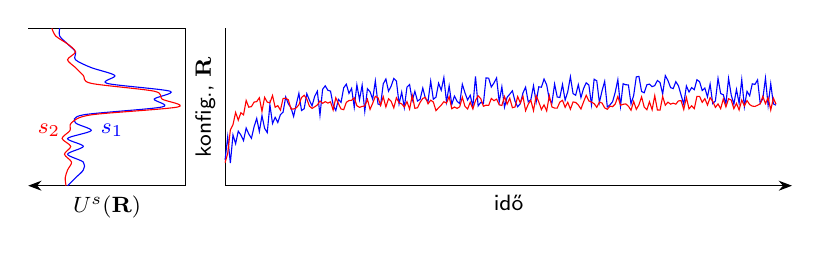
\begin{tikzpicture}[font=\footnotesize]

\draw[-Stealth] (0,-1) -- node[anchor=north] {idő} (7.2,-1) ;
\draw[xshift=-0.0 cm] (0,-1) -- node[rotate=90, anchor=south]
{konfig., \(\mathbf{R}\)} (0,1) ;
\draw[-Stealth, xshift=-0.5 cm] (0,-1) -- node[anchor=north] {\(U^s(\mathbf{R})\)} (-2,-1) ;
\draw[xshift=-0.5 cm] (0,1) -- (-2,1) ;
\draw[xshift=-0.5 cm] (0,-1) -- (0,1) ;

\begin{scope}[rotate=90, yshift=0.5 cm]
% energy landscape
\draw[blue] plot[smooth] coordinates {
(-1.0,1.5) (-0.9,1.4) (-0.8,1.3) (-0.7,1.3) (-0.6,1.5) (-0.5,1.3) (-0.4,1.5)
(-0.3,1.2) (-0.2,1.4) (-0.1,1.3) (0.0,0.3) (0.1,0.4) (0.2,0.2) (0.3,1.0) (0.4,0.9) (0.5,1.2) (0.6,1.4) (0.7,1.4) (0.8,1.5) (0.9,1.6) (1.0,1.6)
};

\node[anchor=west, blue] at (-0.3,1.2) {\(s_1\)};

%\draw[decorate, decoration=brace, gray] (-0.05,1.0) -- node[anchor=east,
%align=right] {native conform.} (0.25,1.0)
%;

\end{scope}

% MD trajectory
\draw[blue, domain=0:7, samples=210]
plot (\x, {- 0.8 * exp(-1.5 * \x) + 0.2 * rand + 0.2 }) 
;
%\draw[decorate, decoration=brace, gray] (0.10,0.5) -- node[anchor=south] {folding} (2,0.5) ;
%\draw[decorate, decoration=brace, gray] (2.10,0.5) -- node[anchor=south]
%{native dynamics} (7,0.5) ;

% another system (red)
\begin{scope}[red]

% MD trajectory
\draw[domain=0:7, samples=210]
plot (\x, {- 0.8 * exp(-10 * \x) + 0.1 * rand + 0.05 }) 
;

\begin{scope}[rotate=90, yshift=0.5 cm]
% energy landscape
\draw plot[smooth] coordinates {
(-1.0,1.52) (-0.9,1.53) (-0.8,1.5) (-0.7,1.45) (-0.6,1.54) (-0.5,1.46)
(-0.4,1.57)
(-0.3,1.47) (-0.2,1.45) (-0.1,1.2) (0.0,0.1) (0.1,0.3) (0.2,0.4) (0.3,1.2)
(0.4,1.3) (0.5,1.4) (0.6,1.5) (0.7,1.4) (0.8,1.5) (0.9,1.65) (1.0,1.7)
};

\node[anchor=east] at (-0.3,1.47) {\(s_2\)};

\end{scope}

\end{scope}

\end{tikzpicture}

\end{document}
